\documentclass[pdf,notes]{beamer}
\mode<presentation>{\usetheme[secheader]{Boadilla}}
\usepackage{mystyle}
\includecomment{versiona}
\usepackage{xeCJK}

\newcommand{\red}[1]{{\color[rgb]{0.6,0,0}#1}}
\setCJKmainfont[AutoFakeBold=true]{Hiragino Mincho Pro} %my Mac
%\setCJKmainfont{MS PGothic} %AJP windows

\makeatletter
\newenvironment<>{proofs}[1][\proofname]{\par\def\insertproofname{#1\@addpunct{.}}\usebeamertemplate{proof begin}#2}
{\usebeamertemplate{proof end}}
\makeatother

\makeatletter
\def\th@mystyle{%
\normalfont % body font
\setbeamercolor{block title example}{bg=orange,fg=white}
\setbeamercolor{block body example}{bg=orange!20,fg=black}
\def\inserttheoremblockenv{exampleblock}
}
\makeatother

\theoremstyle{mystyle}
\newtheorem{prop}{Proposition}

\title{Hermitian Neural Networks}
\subtitle{joint with 小林俊行}
\author{レオンチエフ・アレックス、東大数理}

\begin{document}
\begin{frame}\titlepage\end{frame}
\begin{frame}{Outline}
\tableofcontents
\end{frame}
\newcommand{\mytime}[1]{(#1{分})}
\section{Intro: Orthogonal Neural Networks}
\begin{frame}
	\begin{figure}[h]
		\centering
		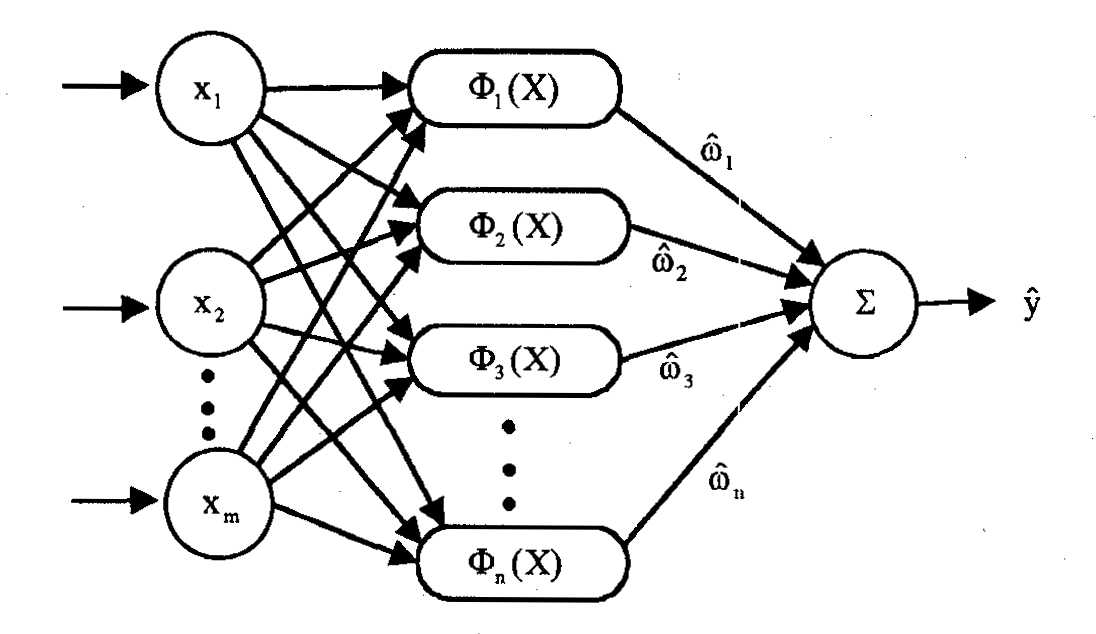
\includegraphics[scale=0.3]{onn}
		\caption{tesime}
		\label{fig:onn}
	\end{figure}
\end{frame}
\section{Intro: Hermitian Neural Networks}
\section{Intro: Hermite-Rodriguez Networks}
\section{My contribution}
\section{Further work}
\section{Q\&{A}\mytime{20}}
\begin{frame}
	\begin{center}
		\Huge Q\&{A}
	\end{center}
\end{frame}
\begin{frame}[allowframebreaks]
\frametitle{References}
\nocite{mackenzie2003hermite}
\nocite{yang1996orthogonal}
\bibliographystyle{amsalpha}
\bibliography{fmsp.bib}
\end{frame}
\end{document}
